
\chapter{Schüler Game Teachify Bird}
Christian Pöhlamnn

\section{Konzept und Spielidee}
Die Grundidee war eine Spielvariante auf der Basis von FlabbyBird zu entwickeln.
Bei FlabbyBird geht es darum einen Vogel an Hindernissen, die sich von rechts nach links über den Bildschirm bewegen vorbei zu navigieren. Durch tippen auf dem Bildschirm wird die Höhe des Vogels beeinflusst, der sich an einer festen Position befindet, und von den sich bewegenden Hindernissen getroffen werden kann.
In unserer Spielvariante wird eine englische Vokabel vorgegeben, und der Spieler muss den Vogel von einer Auswahl an deutschen Vokabeln durch die richtig übersetze Vokabel navigieren. Bei der richtigen Antwort erhält der Spieler Punkte, bei der falschen verliert er Leben.
Ziel des Spieles ist es soviel Punkte wie möglich zu sammeln.

\begin{figure}[H]
	\centering
  \frame{ 
  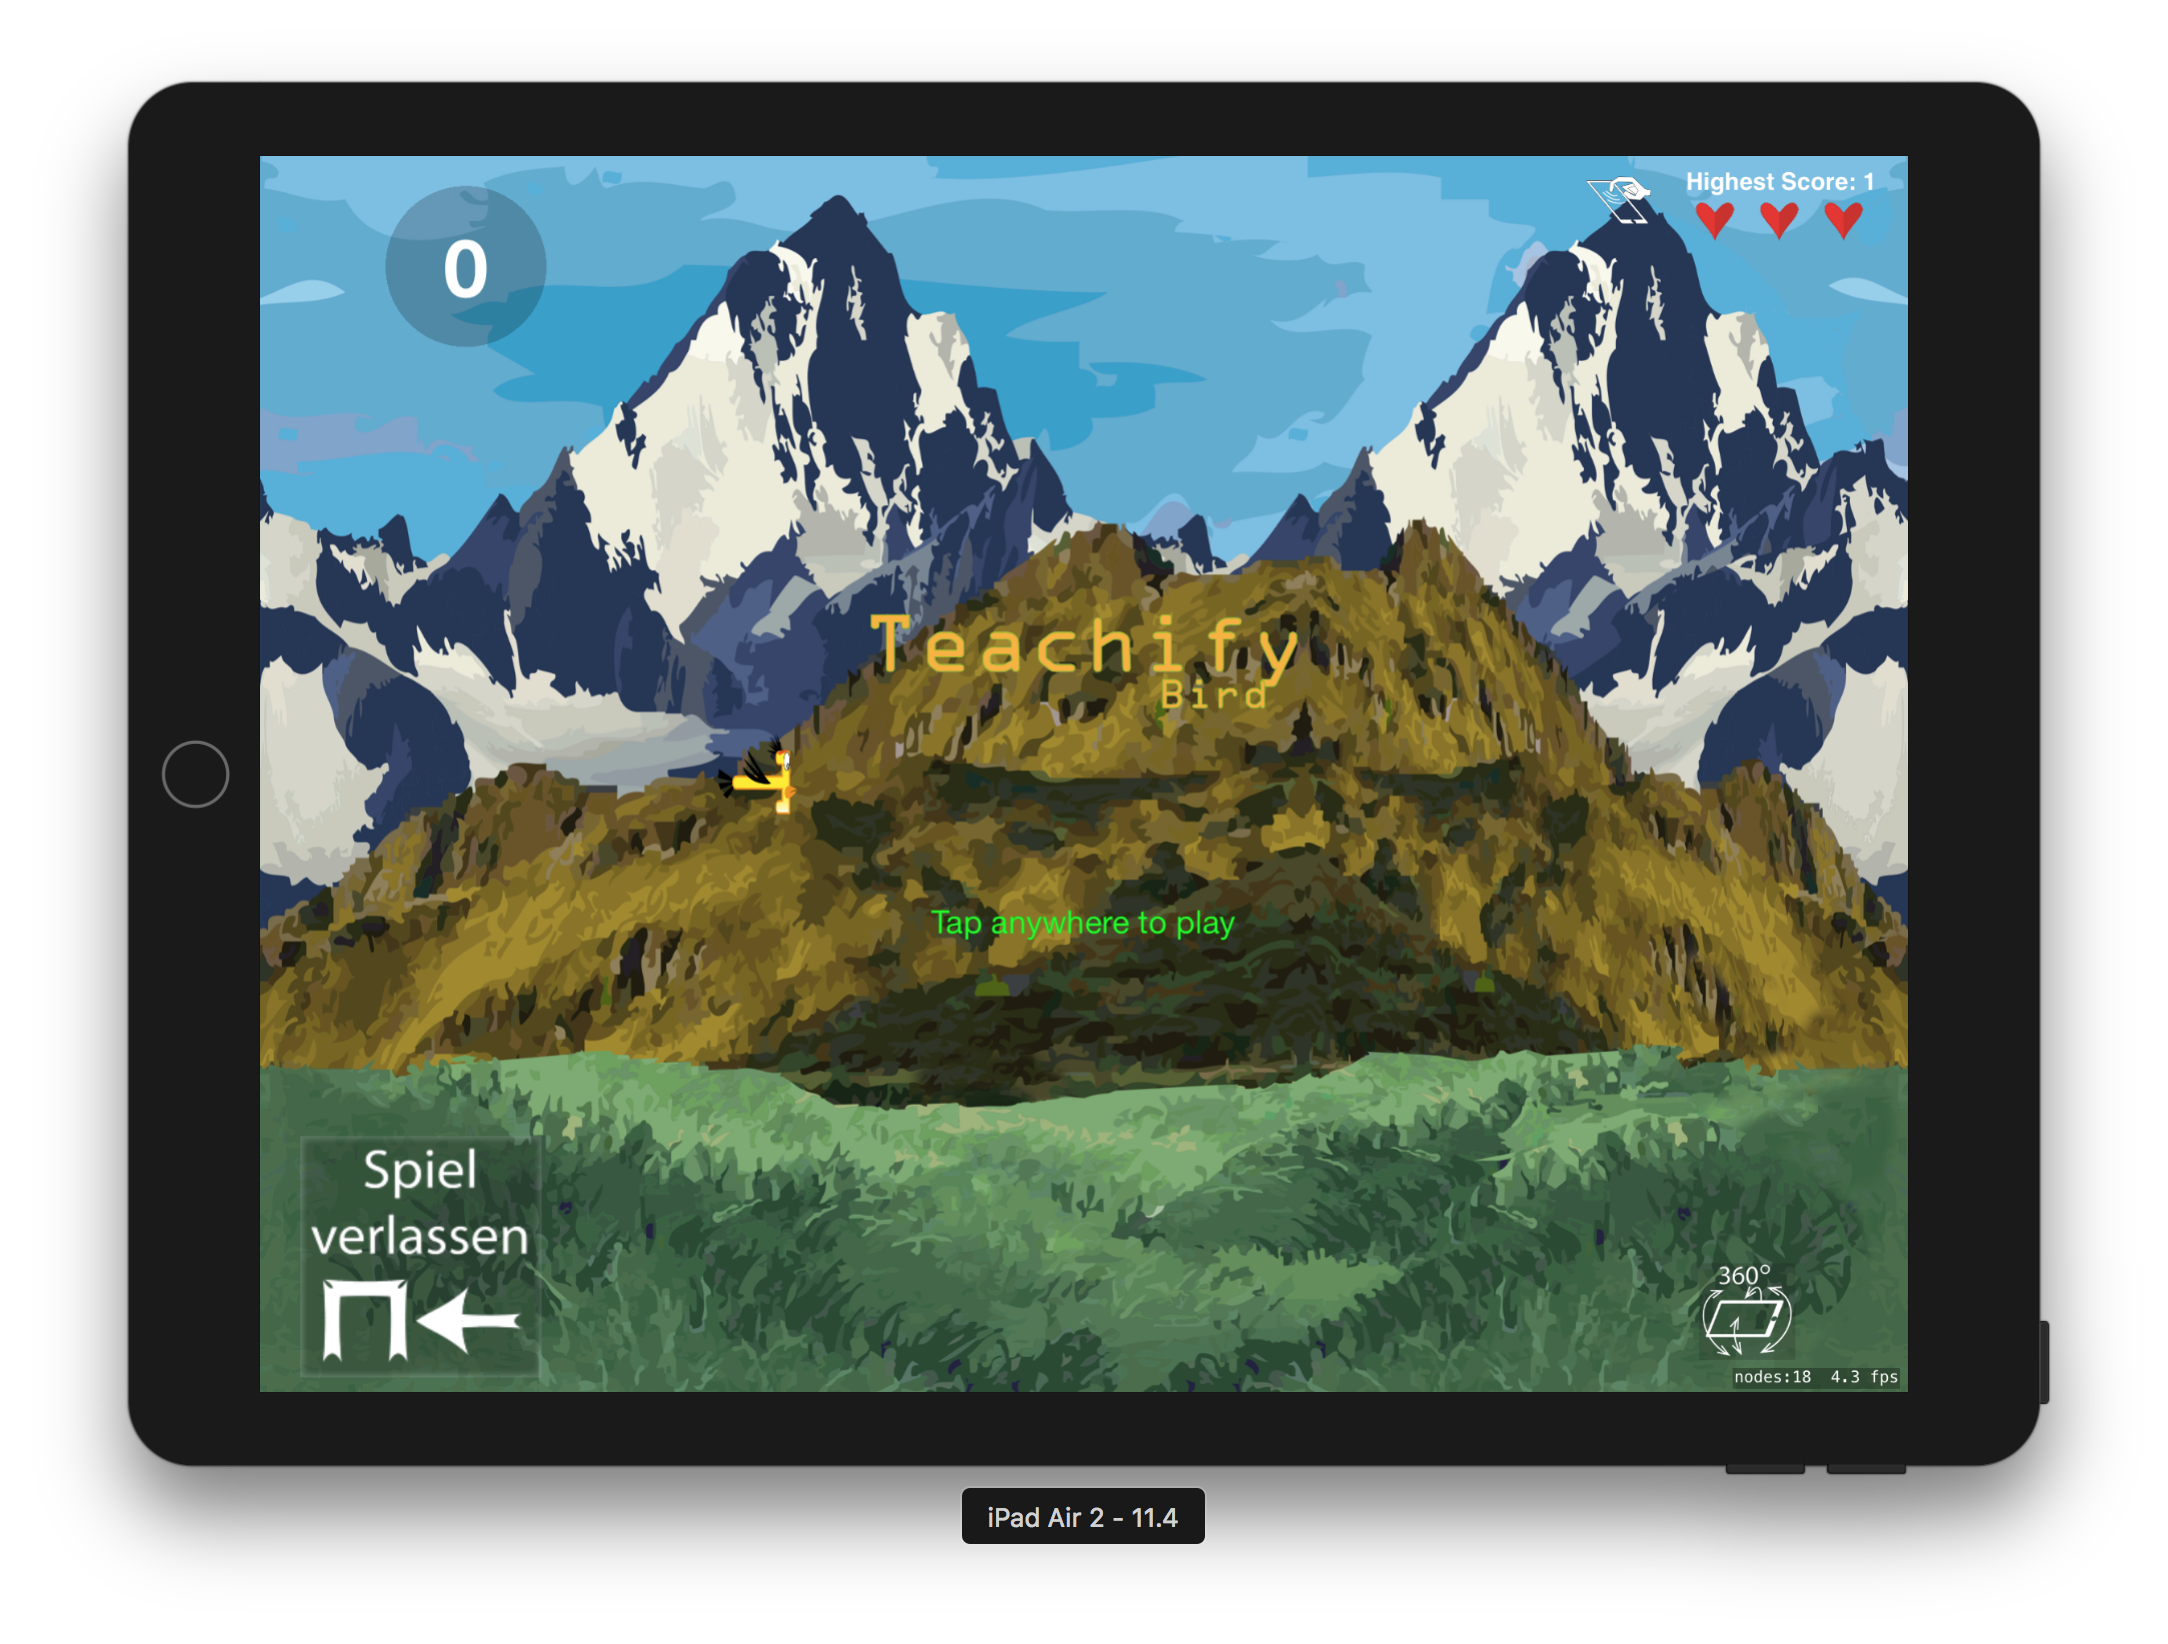
\includegraphics[width=1\textwidth]{images/teachBirdI.png}
  }
	\caption{Teachify Bird Spiel StartScreen}
	\label{Der Login Bildschirm}
\end{figure}

\begin{figure}[H]
	\centering
  \frame{ 
  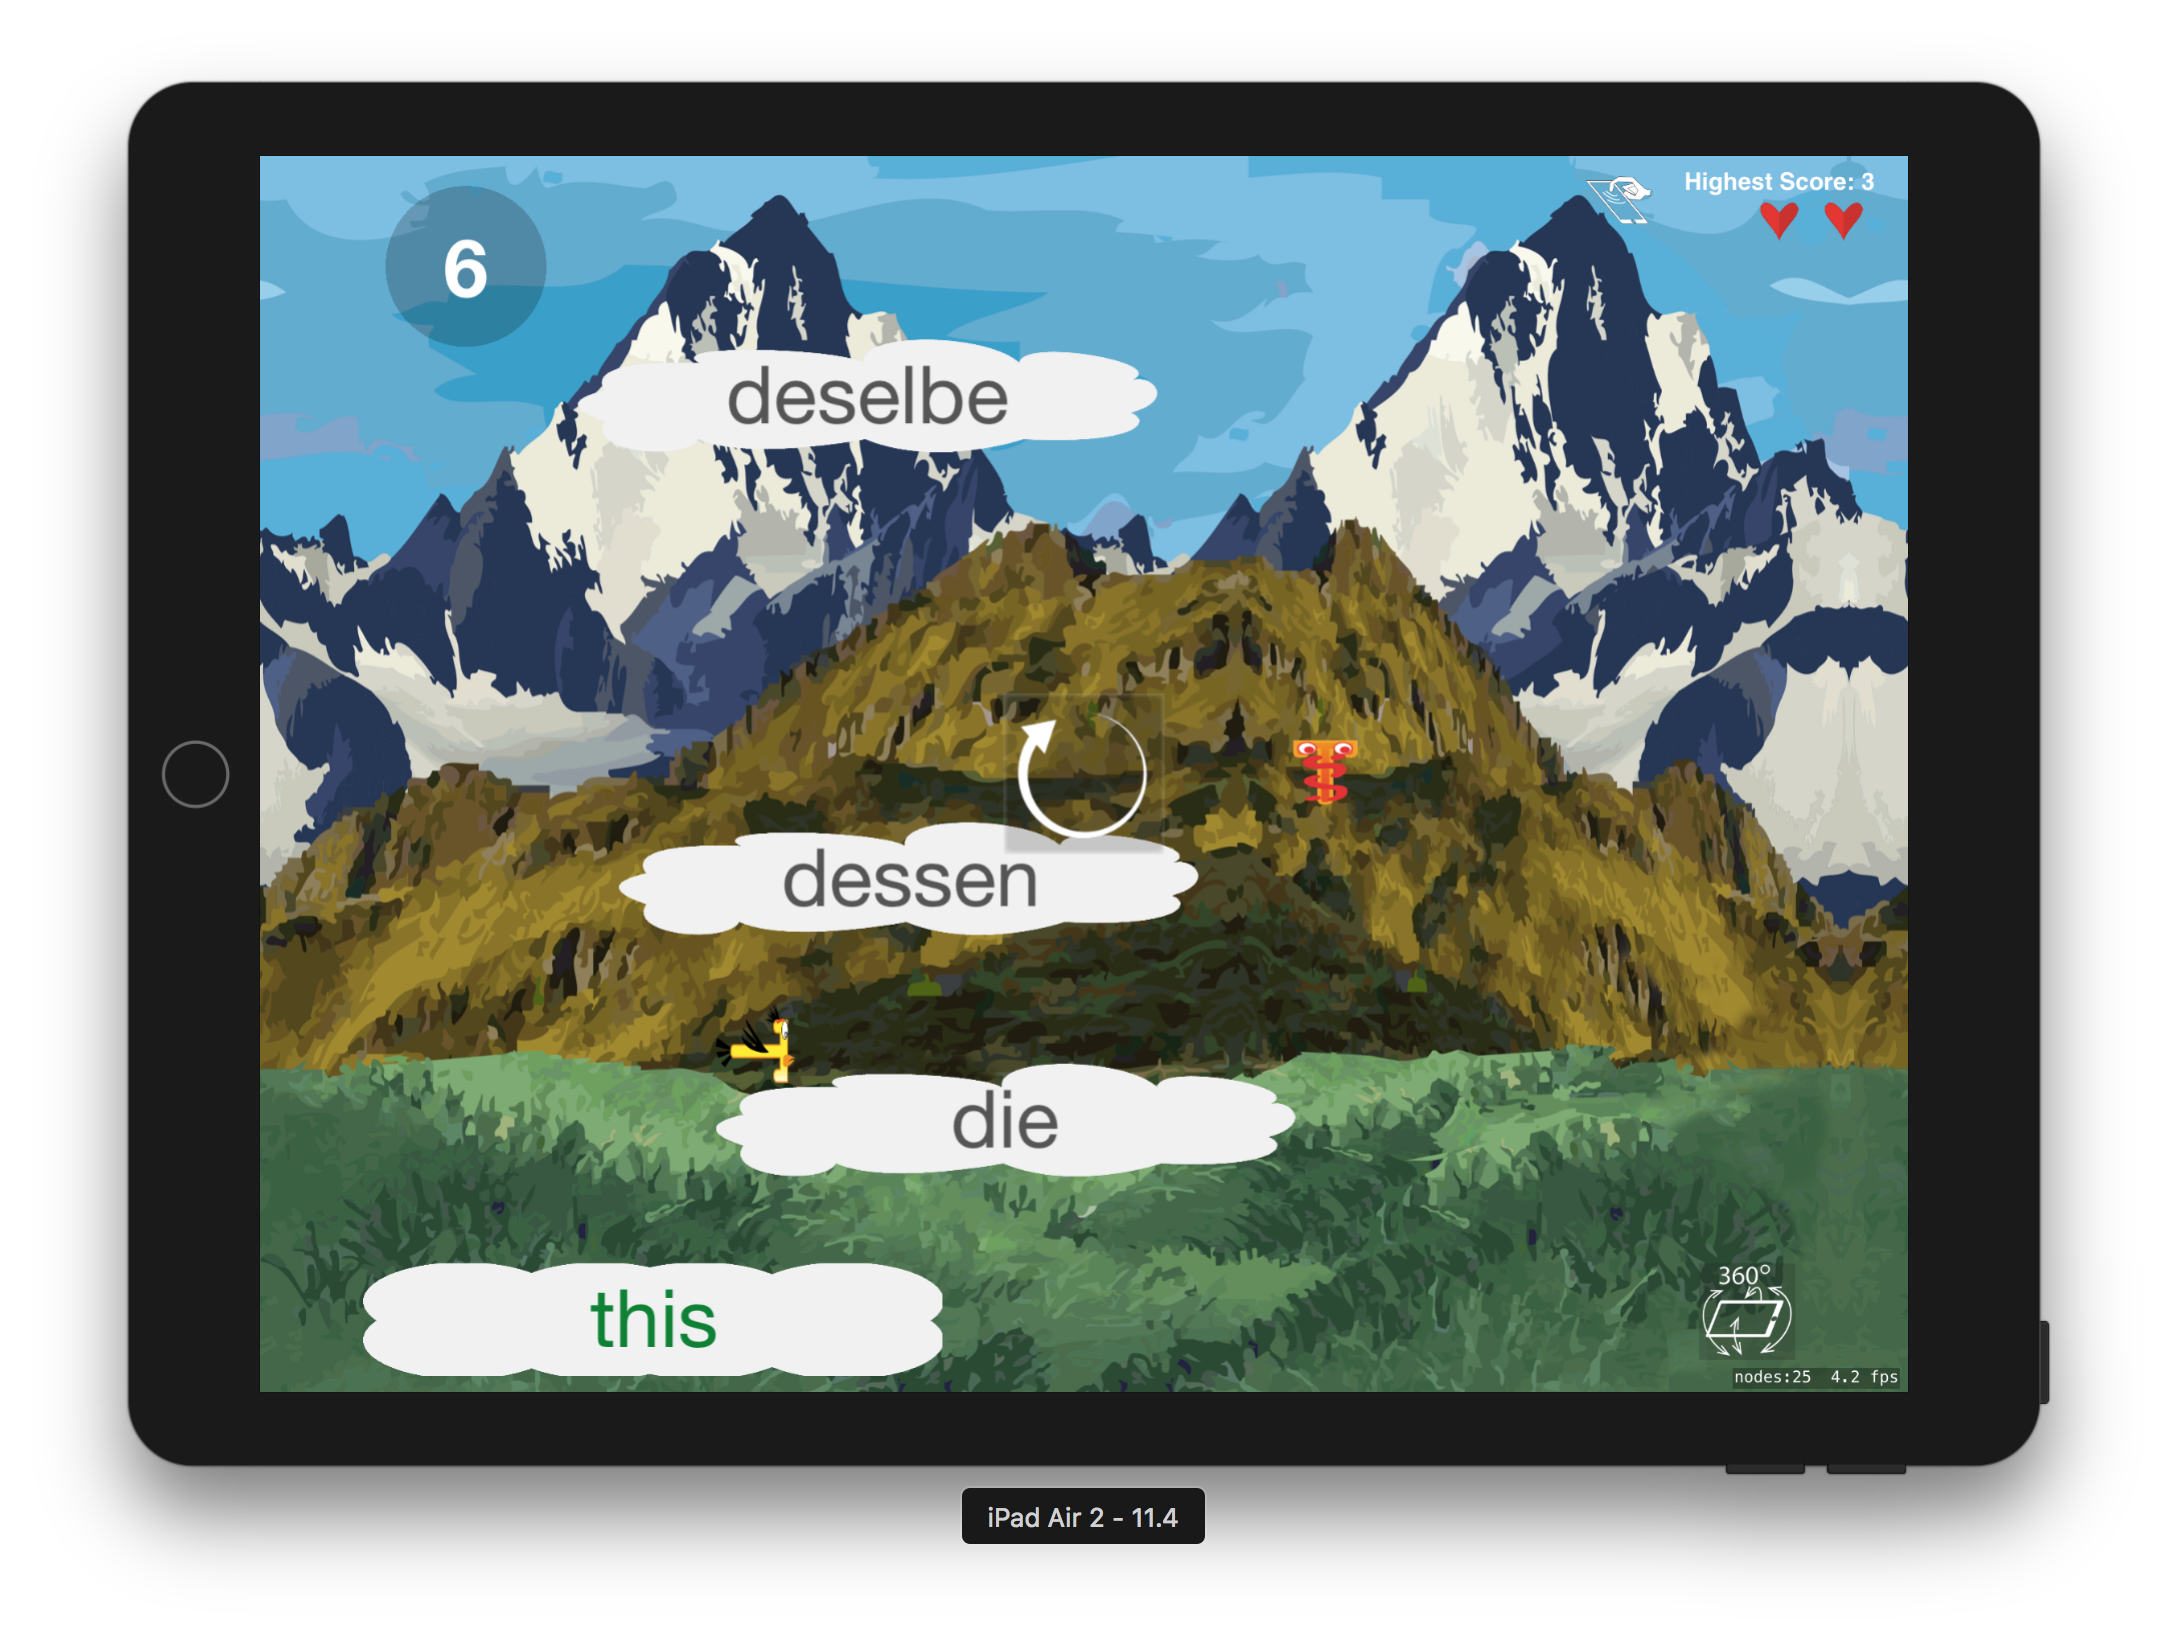
\includegraphics[width=1\textwidth]{images/teachBird.png}
  }
	\caption{Teachify Bird Spiel}
	\label{Der Login Bildschirm}
\end{figure}

\section{Technische Umsetzung}
Umgesetz wurde dieses Spiel mit dem SpriteKit und Swift 4. Für die Spielvariante mit der Gerätebewegung wir ein physisches iPad benötigt.


\section{Aufgaben}
Es wird eine englische Vokabel angezeigt, als Übersetzung gibt es vier deutsche Begriffe, von denen einer die richtige Übersetzung ist. Die Antworten werden in einem geringen Abstand zueinander leicht versetzt übereinander angeordnet. Die richtige Antwort erhält eine zufälligen Position, um den Spieler zum nachdenken zu ermutigen.
Die Antworten bewegen sich von rechts nach links, und der Spieler kann die richtige Antwort durchfliegen, und einen Punkt sammeln, oder an einer falschen Antwort ein Leben verlieren. Die Aufgabenstellung wird so lange die Aufgabe gültig ist unten links konstant angezeigt.
Ist ein Aufgeben-Set zu drei viertel über den Bildschirm gelaufen, wird es gegen einer neuen Aufgabe ersetzt.
Zu jedem Aufgaben-Set gibt es einen Bonuspunkt der eingesammelt werden kann.

\section{Animieren des Backgrounds}
Um eine Flugbewegung des Vogels zu verdeutlichen bewegt sich das Hintergundbild in einer langsamen Geschwindigkeit von rechts nach links. Um die Hintergrundlandschaft realistischer wirken zu lassen wird der Vordergrund der Landschaft langsamer bewegt als dieser Hintergrund. Für die Länge der Landschaft wiederhohlen sich die Hintergrundbilder.

\section{Navigieren des Vogels durch Neigen des Gerätes}
Als alternative zu der mühsamen Steuerung des Birds durch tippen auf dem Bildschirm wurde die Steuerung durch neigen des Gerätes eingeführt. Das Bird kann durch auf und abwärts neigen des Gerätes nach oben und unten gesteuert werden. Zusätzlich kann durch neigen nach links und rechts innerhalb des Bildschirms vorwärts und rückwärts geflogen werden.
Beim Starten des Spieles wird die aktuelle Lage des Gerätes vom Sensor ausgelesen und als Nullstellung verwendet. Die Nullstellung wird nur bei der Horizontalachse je nach Gerätelage kalibriert. Die Steuerung kann über einen Buttons rechts unten vor starten eines Spieles zwischen Tab- und Sensor- Steuerung umgeschaltet werden. Der Aktive Bedienungsmodus wird oben rechts angezeigt. Ist im Hauptmenü der Sensor aktiv, wird das TeachifyBird Logo durch neigen des Gerätes bewegt. Für die Sensor-Steuerung wird CoreMotion verwendet. 

\section{Punkte und Leben}
Ein Spiel hat vier Leben, welche oben rechts als Symbole angezeigt werden. Wird eine Antwort durch umfliegen der Aufgabe ausgelassen, werden zwei Punkte abgezogen. Bei weniger als zwei Punkte wird ein Leben abgezogen.

\section{Animieren des Vogels}
Um das Bird lebendig zu gestalten wurde es animiert und die Flügel in Bewegung versetzt.

\section{Quellenangaben}
\begin{itemize}
    \item Backgroundmusic \linebreak
    https://www.bensound.com/royalty-free-music/track/ukulele
    \item Coin-Sound \linebreak
    http://soundbible.com/free-sound-effects-3.html Must Credit
    \item Died-Sound \linebreak
	https://www.cayzland.de Music Explosion
\end{itemize}
























